\documentclass[a4paper,ngerman, 11pt, DIV11]{scrartcl}
%\documentclass[a4paper,ngerman, 11pt, pagesize]{report}

%% Päambel
\usepackage[T1]{fontenc}
\usepackage[utf8]{inputenc}
\usepackage{babel}

\usepackage{cite}
\usepackage{xcolor}
\newcommand\Diskussionspunkt[1]{\textcolor{red}{#1}}
\usepackage{ulem}

\usepackage{url}
% keine rote Rahmen um die Links anzeigen
\usepackage[pdfborderstyle={/S/U/W 0}]{hyperref}
%\usepackage{hyperref}

% Grafikpaket laden
\usepackage{graphicx}

% Tabellen
\usepackage{booktabs}
\usepackage{longtable}

% pdf einbinden (A3)
\usepackage{nextpage}
\usepackage{afterpage}
\usepackage{pdfpages}
\usepackage{typearea}
\usepackage{pdfpages}

\usepackage{lscape}


% Quelltext
\usepackage{listings}
 \usepackage{color}
 
 \definecolor{middlegray}{rgb}{0.5,0.5,0.5}
 \definecolor{lightgray}{rgb}{0.8,0.8,0.8}
 \definecolor{orange}{rgb}{0.8,0.3,0.3}
 \definecolor{yac}{rgb}{0.6,0.6,0.1}
 
  \lstset{
   basicstyle=\scriptsize\ttfamily,
   keywordstyle=\bfseries\ttfamily\color{orange},
   stringstyle=\color{green}\ttfamily,
   commentstyle=\color{middlegray}\ttfamily,
   emph={square}, 
   emphstyle=\color{blue}\texttt,
   emph={[2]root,base},
   emphstyle={[2]\color{yac}\texttt},
   showstringspaces=false,
   flexiblecolumns=false,
   tabsize=2,
   numbers=left,
   numberstyle=\tiny,
   numberblanklines=false,
   stepnumber=1,
   numbersep=10pt,
   xleftmargin=15pt
 }


%%  Variablen
\newcommand{\authorName}{Ladina Bilgery \and Thomas Wieling}
\newcommand{\auftraggeber}{Interessengemeinschaft Wetterstation Arbon}
\newcommand{\auftragnehmer}{Interstaatliche Hochschule für Technik NTB}
\newcommand{\projektName}{Multiplattform-fähiges und barrierefreies User Interface und Datenmanagement für die Wetterstation Arbon}
\title{\projektName~(Bachelorarbeit)}
\author{\authorName}
\date{\today}

%%  Create a shorter version for tables. DO NOT CHANGE 
\newcommand\addrow[2]{#1 &#2\\ }
\newcommand\addheading[2]{#1 &#2\\ \hline}
\newcommand\tabularhead{\begin{tabular}{lp{13cm}}
\hline
}
\newcommand\addmulrow[2]{ \begin{minipage}[t][][t]{2.5cm}#1\end{minipage}
   &\begin{minipage}[t][][t]{8cm}
    \begin{enumerate} #2   \end{enumerate}
    \end{minipage}\\ }
\newenvironment{usecase}{\tabularhead}
{\hline\end{tabular}}


% damit Bilder im aktuellen Kapitel dargestellt werden
\usepackage{placeins}
\usepackage{geometry}



%%  Beginn Dokument
\begin{document}
\pagenumbering{roman}
\begin{titlepage}
\maketitle
\thispagestyle{empty} 

\begin{verbatim}

\end{verbatim}


  \begin{tabular}[t]{ll}
	Projekt:       & \quad \projektName \\[1.2ex]
	Auftraggeber:  & \quad \auftraggeber\\[1.2ex]
	Auftragnehmer: & \quad \auftragnehmer\\[1.2ex]
  \end{tabular}

\begin{tabular}{|p{3 cm}|p{3 cm}|p{5 cm}|}
\hline
\textbf{Version} & \textbf{Datum} & \textbf{Autor(en)} \\
\hline
\hline
1.0 & 16.11.2017 & \authorName \\
\hline
\end{tabular}
\end{titlepage}

\setcounter{page}{2}
\tableofcontents          
\clearpage
\pagenumbering{arabic}

%%%%%%%%%%%%%%%%%%%%%%%%%%%%%%%%%%%
%%  Einführung
%%%%%%%%%%%%%%%%%%%%%%%%%%%%%%%%%%%
\section*{Einführung ins Thema}

Die Wetterstation Arbon wurde 2005 als Lehrlingsarbeit des Berufsbildungszentrums Arbon auf Initiative der Technischen Gesellschaft Arbon (TGA) aufgebaut und in Betrieb genommen. Sie besteht aus mehreren Wettersensoren und einer Webcam, die auf einer Plattform auf dem See draussen montiert sind. Die Messwerte werden auf der Webseite\footnote{ \url{https://www.wetter-arbon.ch}}  der Wetterstation Arbon angezeigt.

\begin{figure}[h!]
	\centering
	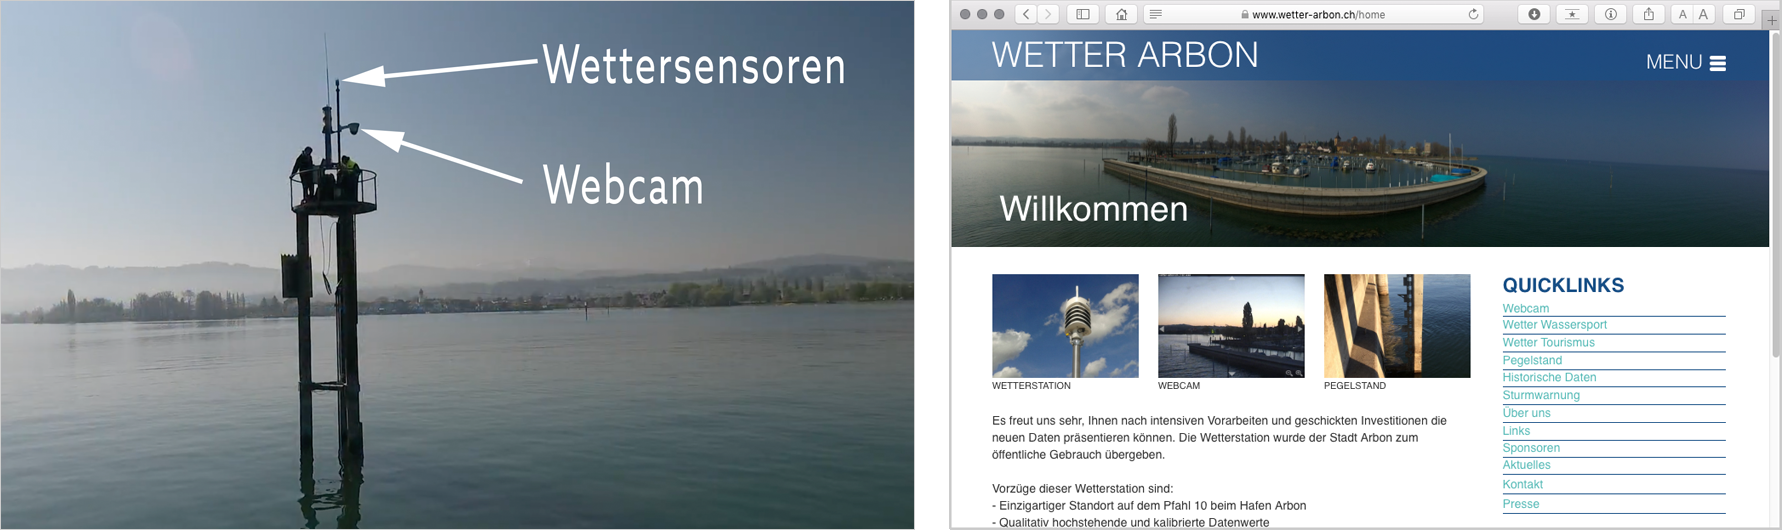
\includegraphics[width=1\linewidth]{img/kombi}
	\caption{Installation und Webseite der Wetterstation Arbon}
	\label{img:wetterstation}
\end{figure}

Was damals modern war, ist heute veraltet. Sowohl auf der Hardwareseite, als auch auf der Webseite gibt es diverses Reparatur- beziehungsweise Modernisierungspotential. Die Bachelor-Arbeit hat das Ziel die Wetterstation wieder auf einen modernen, vollfunktionsfähigen Stand zu bringen. Während des Fachmoduls, welches die Vorbereitung für die Bachelor-Arbeit darstellt, führten wir eine Ist-Aufnahme der Wetterstation Arbon durch. Im Fokus lag sowohl die Hardware als auch die Software. Der Übersicht halber und damit wir die Arbeiten besser untereinander aufteilen konnten, haben wir die Themen in die vier Blöcke:  Webseite, Datenbank, Sensoren und Webcam unterteilt. (vgl. Abb. \ref{img:module})

\vspace{5mm} %5mm vertical space

\begin{figure}[h!]
	\centering
	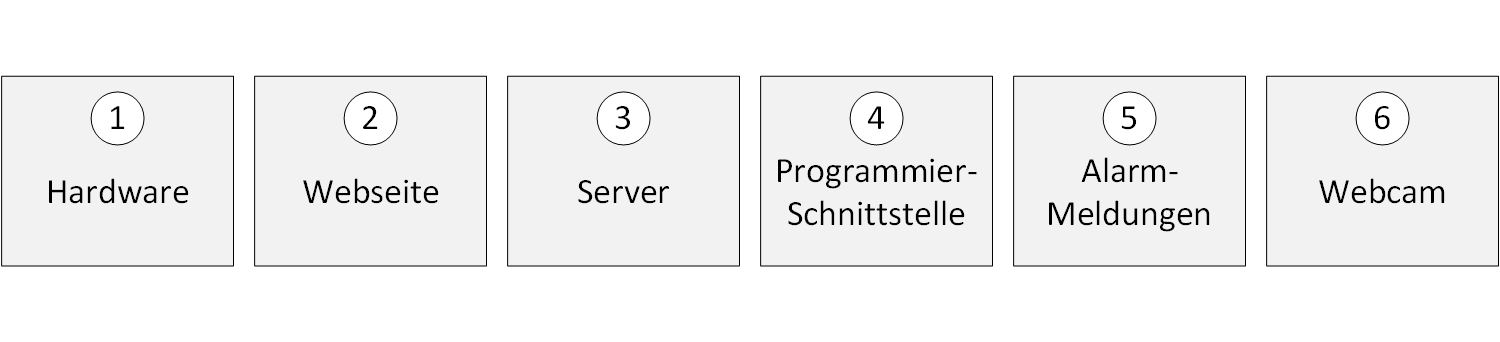
\includegraphics[width=0.8\linewidth]{img/module}
	\caption{Aufteilung in Arbeitsblöcke}
	\label{img:module}
\end{figure}

Dieser Bericht zeigt jeweils pro Block auf, wie die jetzige Situation ist, wo die Problemstellen liegen, wie diese behoben werden können und was die Anforderungen an die Lösung ist. Die Erkenntnisse des Fachmoduls dienen als Grundlage für die Bachelor-Arbeit. Dort geht es darum die Lösungsansätze zu konkretisieren und umzusetzen.

\newpage
\section*{Zusammenfassung}
\Diskussionspunkt{- Kapitel muss noch erstellt werden}\newline
\Diskussionspunkt{- Schlussfolgerung / Aussichten / weitere Schritte}\newline
\Diskussionspunkt{- Was waren die grössten Herausforderungen / was könnte besser gemacht werden}\newline
\Diskussionspunkt{- Was konnte umgesetzt werden}\newline
\Diskussionspunkt{- Welche Anforderungen wurden nicht erfüllt}\newline

\section{Datenbank}

\Diskussionspunkt{Beginn Einlesen in DB}
Verschiedene Arten von Datenbanken:
\begin{itemize}
\item relationale DB
\item hierarchisches Datenmodell
\item Netzwerkdatenmodell
\item Objekt relationale Datenbank
\end{itemize}

Das relationale Datenmodell ist das weit verbreiteste Modell, dass hierarchische wegen der beschränkten Anwendbarkeit kaum noch vorhanden.

Vorgehen Datenbankentwicklung:

\begin{itemize}
\item Externe Phase (Ermittlung der Informationsstruktur)
\item Konzeptionelle Phase (ER-Modell)
\item Logische Phase (relationales Datenmodell)
\item Physische Phase (Erstellung des Datenmodell)
\end{itemize}

Punkte zur Überlegung neuer Datenbankstruktur:
\begin{itemize}
\item Welche Daten?
\item In welchem Intervall?
\item Welche Tabellen? (Welche Daten zusammen?, eine grosse Tabelle?)
\item Tabellennamen?
\item 
\end{itemize}

https://entwickler.de/online/datenbanken/datenbanken-grundlagen-und-entwurf-115676.html
\Diskussionspunkt{Ende Einlesen in DB}

\section{Kapitel 2}
blabla 
\section{Barrierefreiheit}

Denn von einer verbesserten Zugänglichkeit profitieren nicht nur Menschen mit Einschränkungen, sondern auch die Informationsanbieter durch die Ansprache von Millionen zusätzlicher potenziellen Benutzer. Als Bonus kommt eine verbesserte Indizierung durch Suchmaschinen und infolgedessen eine bessere Position im Suchmaschinen-Ranking hinzu.

Im Kern geht es also darum, die Webapplikation so zu gestalten, dass sie möglichst für alle Benutzergruppen zugänglich ist. Dazu zählen nicht nur Menschen mit schweren und permanenten Einschränkungen, Kranke und Verletzte, funktionale Analphabeten und Legastheniker sowie die steigende Zahl an Seniorenauch veraltete Technik oder aber der allerneueste Stand der Technik (mobile Endgeräte wie etwa Tablet PC oder Smartphone) kann zu Schwierigkeiten führen.

hohen Lärmpegel (z. B. in einer Fabrikhalle) oder Zwang zur Stille (z. B. in einer Bibliothek) keine akustische Ausgabe gestatten, die Lichtverhältnisse einen besonders hohen Kontrast erfordern

Eine von Microsoft beauftragte Studie ~\cite{ForresterResearch2004E:Abilities} der \flqq Forrester Research Inc.\frqq schätzt, dass über 60 Prozent aller Computernutzer von Barrierefreiheit profitieren können. 


Gemäss \flqq Interface Design\frqq ~\cite{ThesmannStephan2016ID:U} wird Barrierefreiheit bald Standard sein.







\subsection{Web Content Accessibility Guidelines (WCAG)}

Die aktuellen Web Content Accessibility Guidelines 2.0 (WCAG2) fordern die Einhaltung von vier Designprinzipien:

\begin{itemize}  
\item Prinzip 1: Wahrnehmbarkeit 
\item Prinzip 2: Bedienbarkeit
\item Prinzip 3: Verständlichkeit
\item Prinzip 4: Robustheit
\end{itemize}

Die Ziele dieser vier Prinzipien sind durch zwölf Richtlinien (Guidelines) genauer spezifiziert. Zu jeder Richtlinie geben die WCAG2 testbare Erfolgskriterien (Success Criteria) vor.

Priorität 1 („Muss-Kriterien“): Webauftritte müssen alle A-Anforderungen erfüllen, weil es sonst für eine oder mehrere Benutzergruppen unmöglich wäre, auf die Information im Dokument zuzugreifen.

Priorität 2 („Soll-Kriterien“): Die Erfüllung der AA-Anforderungen beseitigt signifikante Hindernisse und erleichtert einer oder mehreren Benutzergruppen den Zugriff auf Web-Dokumente.

Priorität 3 („Kann-Kriterien“): Diese AAA-Anforderungen können erfüllt werden, um den Zugriff auf Web-Dokumente für eine oder mehrere Benutzergruppen zu erleichtern. Sind die Prioritäten 1 bis 3 erfüllt, erhält das Informationsangebot die Konformitätsstufe AAA.

\subsection{Relevante Anforderungen für die Webseite der Wetterstation}

\subsubsection*{Prinzip 1: Wahrnehmbarkeit}
Anforderung 1.1: Text-Alternativen 
-> für alle Anzeigegrafiken und Bilder
Anforderung 1.2: Zeitbasierte Medien 
-> Film-Aufnahme
Anforderung 1.3: Anpassbarkeit
Anforderung 1.4: Unterscheidbarkeit


\subsubsection*{Prinzip 2: Bedienbarkeit}
Anforderung 2.1: Zugänglichkeit per Tastatur
Anforderung 2.2: Bereitstellung ausreichender Zeit
Anforderung 2.3: Vermeidung von Anfällen
Anforderung 2.4: Navigierbarkeit


\subsubsection*{Prinzip 3: Verständlichkeit}
Anforderung 3.1: Lesbarkeit
Anforderung 3.2: Vorhersehbarkeit
Anforderung 3.3: Hilfestellung bei der Eingabe

\subsubsection*{Prinzip 4: Robustheit}
Anforderung 4.1: Kompatibilität


\subsection{Accessible Rich Internet Applications (WAI-ARIA) 1.1 -> Semantik}

WAI-ARIA ist eine technische Spezifikation, die ein Framework für die Verbesserung der Zugänglichkeit und Interoperabilität von Web-Inhalten und -Anwendungen bietet.

Menschen mit bestimmten Arten von Behinderungen nutzen assistive Technologien (AT), um mit Inhalten zu interagieren. Assistive Technologien können die Präsentation von Inhalten in ein für den Benutzer besser geeignetes Format umwandeln und es dem Benutzer ermöglichen, auf unterschiedliche Weise zu interagieren. Um dies effektiv zu bewerkstelligen, muss die Software die Semantik der Inhalte verstehen. Semantik ist die Wissenschaft der Bedeutung; in diesem Fall wird sie verwendet, um Rollen, Zustände und Eigenschaften zuzuweisen, die für Benutzeroberflächen und Inhaltselemente gelten, wie sie ein Mensch verstehen würde. Rollen sind eine gemeinsame Eigenschaft von accessibility APIs für die Zugänglichkeit, die von assistiven Technologien verwendet werden, um dem Benutzer eine effektive Präsentation und Interaktion zu ermöglichen.

Rollen sind Elementtypen und ändern sich nicht mit der Zeit oder Benutzeraktionen. Rolleninformationen werden von assistiven Technologien durch Interaktion mit dem User-Agent verwendet, um eine normale Verarbeitung des angegebenen Elementtyps zu ermöglichen. Zustände und Eigenschaften werden verwendet, um wichtige Attribute eines Elements zu deklarieren, die die Interaktion beeinflussen und beschreiben. 

Schlagwörter:
accessibility APIs
WAI-ARIA Roles
WAI-ARIA States and Properties

Roles:
Hauptindikator des Typs. Diese semantische Assoziation ermöglicht es den Werkzeugen, die Interaktion mit dem Objekt in einer Weise darzustellen und zu unterstützen, die mit den Erwartungen der Benutzer an andere Objekte dieses Typs übereinstimmt.

Properties:
Attribute, die für die Beschaffenheit eines bestimmten Objekts wesentlich sind oder einen mit dem Objekt verknüpften Datenwert repräsentieren. Eine Änderung einer Eigenschaft kann die Bedeutung oder Präsentation eines Objekts erheblich beeinflussen.


States:
Ein Zustand (state) ist eine dynamische Eigenschaft, die Eigenschaften eines Objekts ausdrückt, die sich als Reaktion auf Benutzeraktionen oder automatisierte Prozesse ändern können. Zustände haben keinen Einfluss auf die essentielle Natur des Objekts, sondern stellen Daten dar, die mit dem Objekt verbunden sind, oder Möglichkeiten der Benutzerinteraktion.

\Diskussionspunkt{https://www.w3.org/TR/wai-aria/#ua_noninterference}

\section{Kapitel4}
\section{Kapitel5}   
\section{Projektmanagement}
Wir wollen das Projektmanagement schlank halten um möglichst viel Zeit in die Entwicklung der Artefakte stecken zu können.
Dieser Grundgedanke hat uns bei der im Folgenden beschrieben Auswahl der Modelle und Prozesse geleitet.

% ################################
% Vorgehensmodell
% ################################
\subsection{Vorgehensmodell}

Die Anforderungen an das Vorgehensmodell haben wir folgendermassen definiert:
\begin{itemize}  
\item wenig administrativer Aufwand, schlank
\item passend zur Projektgrösse
\item kompatibel mit den NTB-Vorgaben (Aufteilung Fachmodul, Bachelor-Arbeit)
\end{itemize}

Schnell merkten wir, dass die heutzutage beliebten agilen Vorgehensmodelle wie XP oder Scrum für uns ein Overkill darstellen und aus mehrerer Hinsicht nicht geeignet sind. Bei der Bachelor-Arbeit sind die Anforderungen im Fachmodul-Bericht definiert und ändern sich während der Bachelor-Arbeit nicht mehr. Die zu bearbeitenden Themen-Blöcke weisen untereinander nur sehr wenige Schnittstellen auf und können dadurch als eigenständige Teilprojekte das Modell durchlaufen. Unser Team besteht zudem nur aus zwei Personen, was den Koordinationsaufwand auf ein minimum reduziert.

\begin{figure}[htbp]
	\centering
	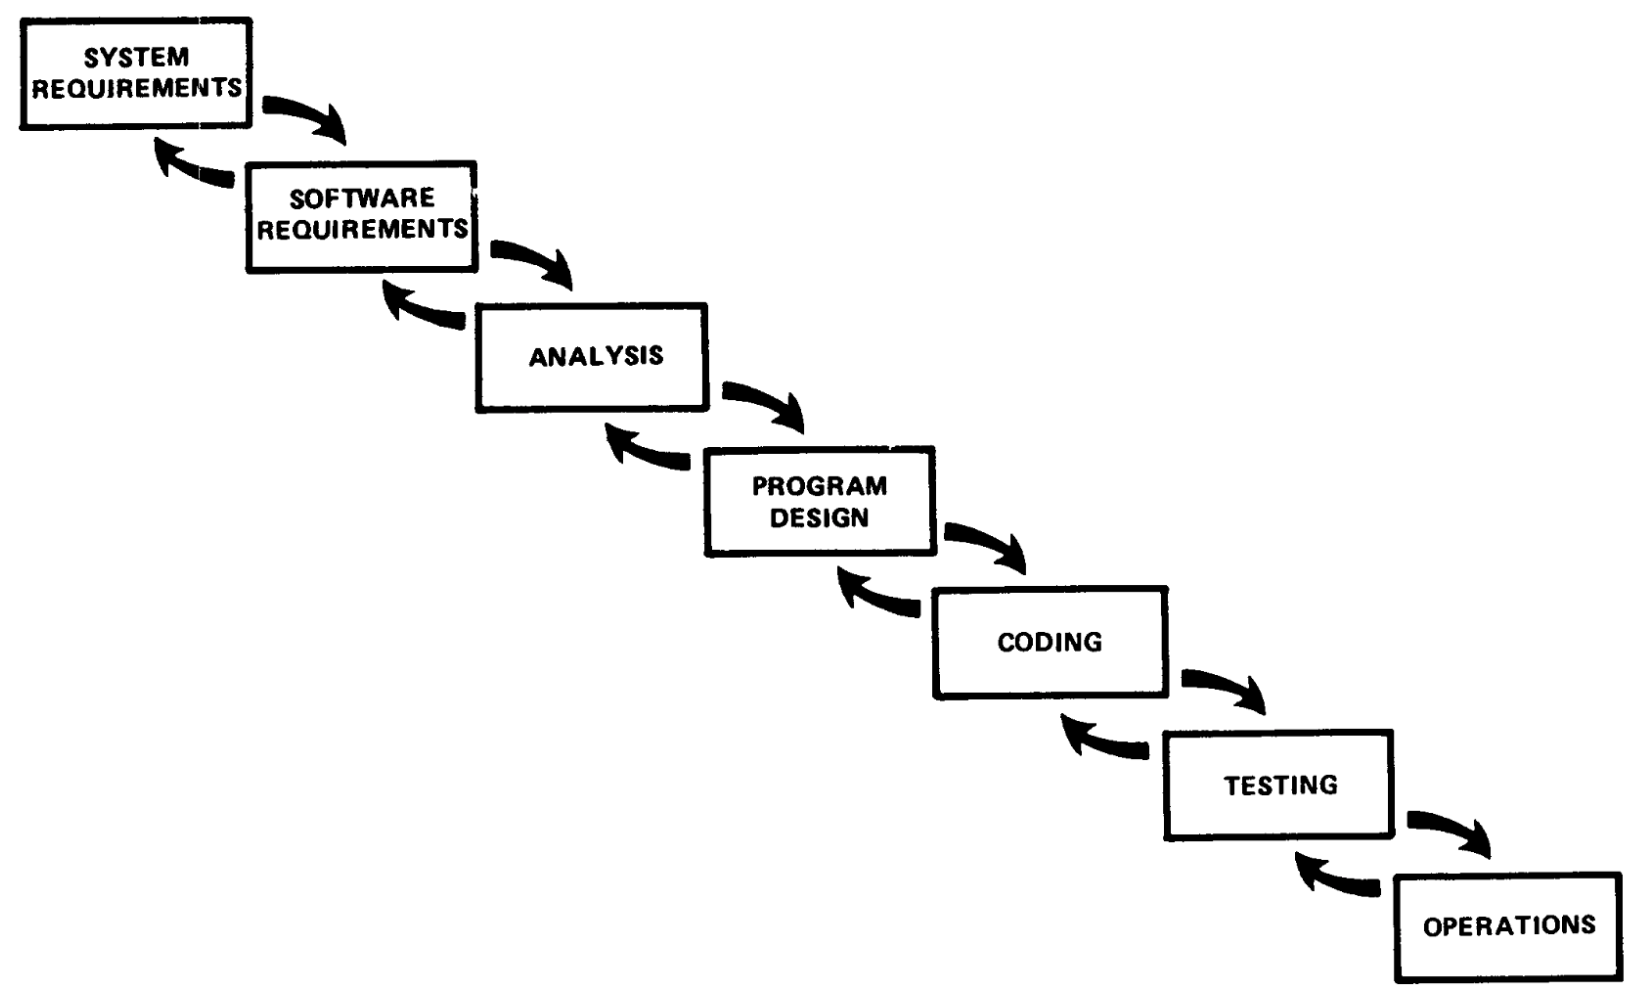
\includegraphics[width=0.9\linewidth]{img/royce-largePrograms}
	\caption{Vorgehensmodell nach Royce}
	\label{img:royce-largePrograms}
\end{figure}


Unsere Bedürfnisse deckt das Vorgehensmodell von Royce ~\cite{Royce1970}, welches in Abbildung  \ref{img:royce-largePrograms} dargestellt ist, am besten ab. Es besteht grundsätzlich aus einem sequentiellen Ablauf der Entwicklungsphasen, berücksichtigt dabei aber auch die Notwendigkeit von Rücksprüngen zur vorherigen Phase.
Die ersten Phasen von der Definition der \textit{System Requirements} bis zu den ersten Gedanken zum Thema \textit{Program Design} behandeln wir im Fachmodul. Der zweite Teil mit der genauen Definition des \textit{Programm Designs} bis zum Betrieb der Software findet anschliessend während der Bachelor-Arbeitszeit statt.


% ################################
% Entwicklungsprozess
% ################################
\subsection{Entwicklungsprozess}
Den Entwicklungsprozess führen wir mit Kanban. Kanban basiert auf dem Pull-Prinzip d.h. jeder, der im Projekt arbeitet, holt sich selbst einen neuen Arbeitsauftrag, sobald er mit einem fertig ist. Die führt dazu, dass die Arbeiten speditiver abgewickelt werden und spart zudem die Stelle des Projektmanagers, der die Aufgaben verteilt.

\begin{figure}[htbp]
	\centering
	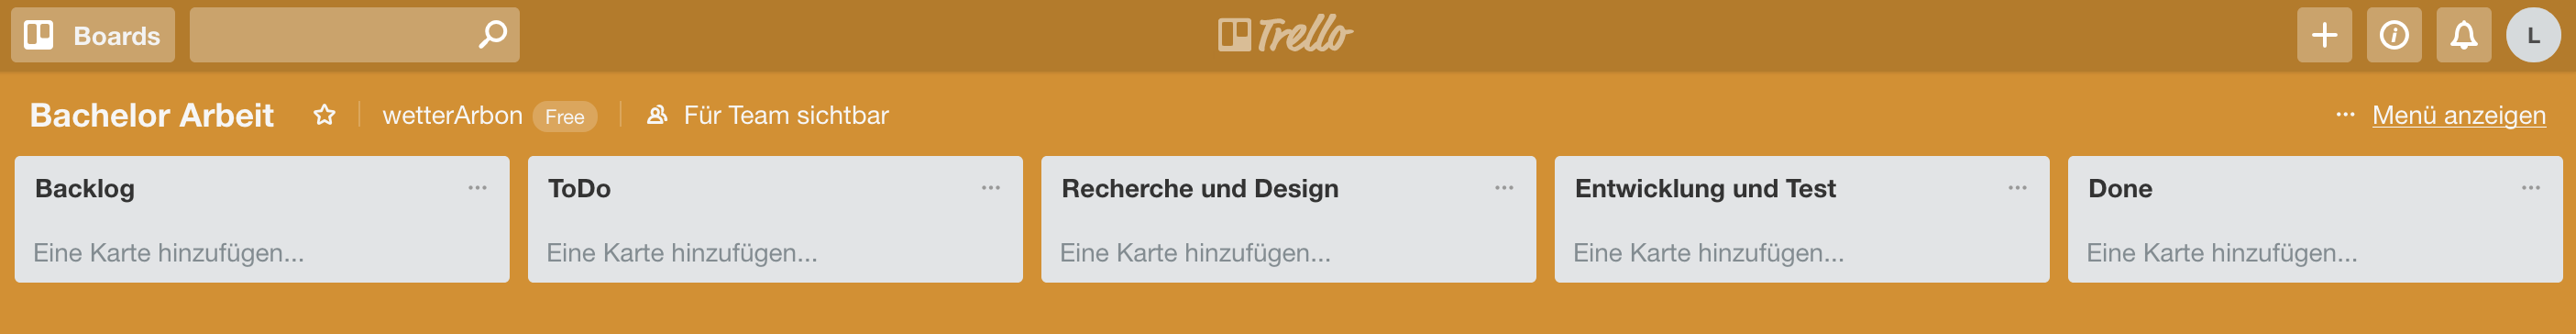
\includegraphics[width=1\linewidth]{img/kanban}
	\caption{Kanban}
	\label{img:kanban}
\end{figure}


David Anderson \cite{AndersonDavidJ2011K:eC} hat das System Kanban, welches ursprünglich aus der Industrie kommt, auf die IT angepasst und dadurch das \textit{Virtuelle Kanban System} entwickelt. Die grundlegenden Regeln daraus lauten:

\begin{itemize}  
\item Jede Karte ist eine Aufgabe
\item Die Aufgabe soll maximal 8 bis16~h benötigen
\item Pro Arbeits-Spalte sind die Anzahl Karten limitiert
\item Eine neue Karte darf erst gezogen werden, wenn die vorherige fertig ist (Multitasking-Vermeidung)
\end{itemize}

% ################################
% Risikoanalyse
% ################################
\subsection{Risikoanalyse}
Für die Risikoanalyse haben wir eine Liste der möglichen  Risiken erstellt. Als Grundlage verwendeten wir das Risikolexikon aus dem Buch \flqq IT-Risikomanagment leben!\frqq ~\cite{AhrendtsFabian2008Il:w}. 
Für jedes Risiko haben wir die Eintretenswahrscheinlichkeit und das Ausmass abgeschätzt. Gegenüber den herkömmlichen Risikobeurteilungen, haben wir allerdings die Auswirkungen auf Kosten und Terminverzug weggelassen, da sie in unserem Projekt nicht relevant sind und uns auf den Stundenaufwand und den Funktionsumfang beschränkt. Um die Auswirkung der einzelen Risiken abschätzen zu können, haben wir eine Punkteskala mit entsprechenden Kriterien erstellt, wie in Tabelle \ref{tab:auswirkung} aufgeführt. \vspace{5mm} %5mm vertical space

\begin{table}[h!]
\centering
\label{tab:auswirkung}
\begin{tabular}{rl}
Wert	[-]	& 	Auswirkung bezüglich Umfang \\
\hline
10	&	Gesamter Block nicht funktionsfähig \\
8	&	Einzelne Funktion nicht umgesetzt  \\
6	&	Bemerkbar, keine Funktionseinbusse \\
4	&	von eingeschränkter Benutzergruppe bemerkbar \\
2	&	von Kunden nicht bemerkbar
\end{tabular}
\end{table}

Die Risikomatrix in Abbildung \ref{img:risikomatrix} zeigt auf grafische Weise wie kritisch die einzelnen Risiken aus der Risikoliste sind. Mindestens vier davon sind als hoch eingestuft und müssen im Rahmen der Bachelor-Arbeit reduziert werden. Dies sind:

\begin{itemize}  
\item Komplexe Datenmigration
\item Mangel an Echtzeitverhalten
\item Mangelnde Ressourcenverfügbarkeit
\item Mangelnde Anforderungsqualität
\end{itemize}


% Abbildung der Risikomatrix
\begin{figure}[h!]
	\centering
	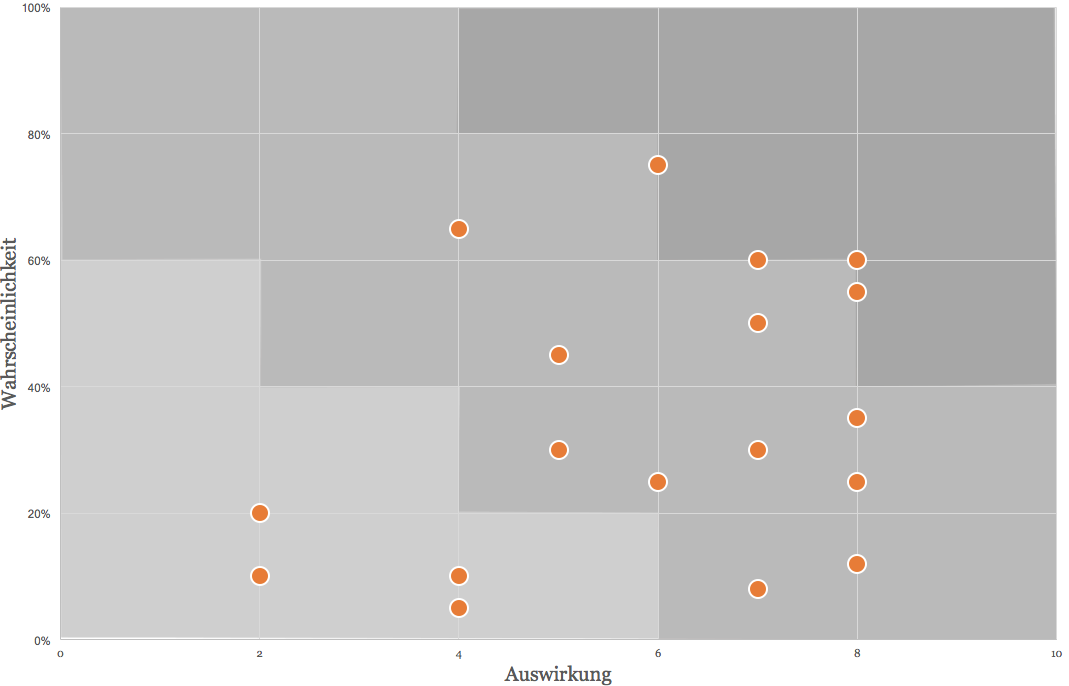
\includegraphics[width=1\linewidth]{img/risikomatrix.pdf} 
	\caption{Risikomatrix}
	\label{img:risikomatrix}
\end{figure}



% ################################
% Projektplan
% ################################

\subsection{Projektplan für die Bachelor-Arbeit}
Der Zeitplan für die Bachelor-Arbeit ist in Abbildung \ref{img:terminplan} auf Seite \pageref{img:terminplan} dargestellt.
Im oberen Teil sind die allgemeinen Termine und Abwesenheiten aufgeführt. Der mittlere Teil zeigt die Arbeitsverteilung über das Semester und am Schluss kommen die Zeitaufwände für Doku und Meetings. Die Dokumentation wollen wir kontinuierlich erstellen, sodass wöchentlich ein entsprechender Block vorgesehen ist.

\begin{figure}[h!]
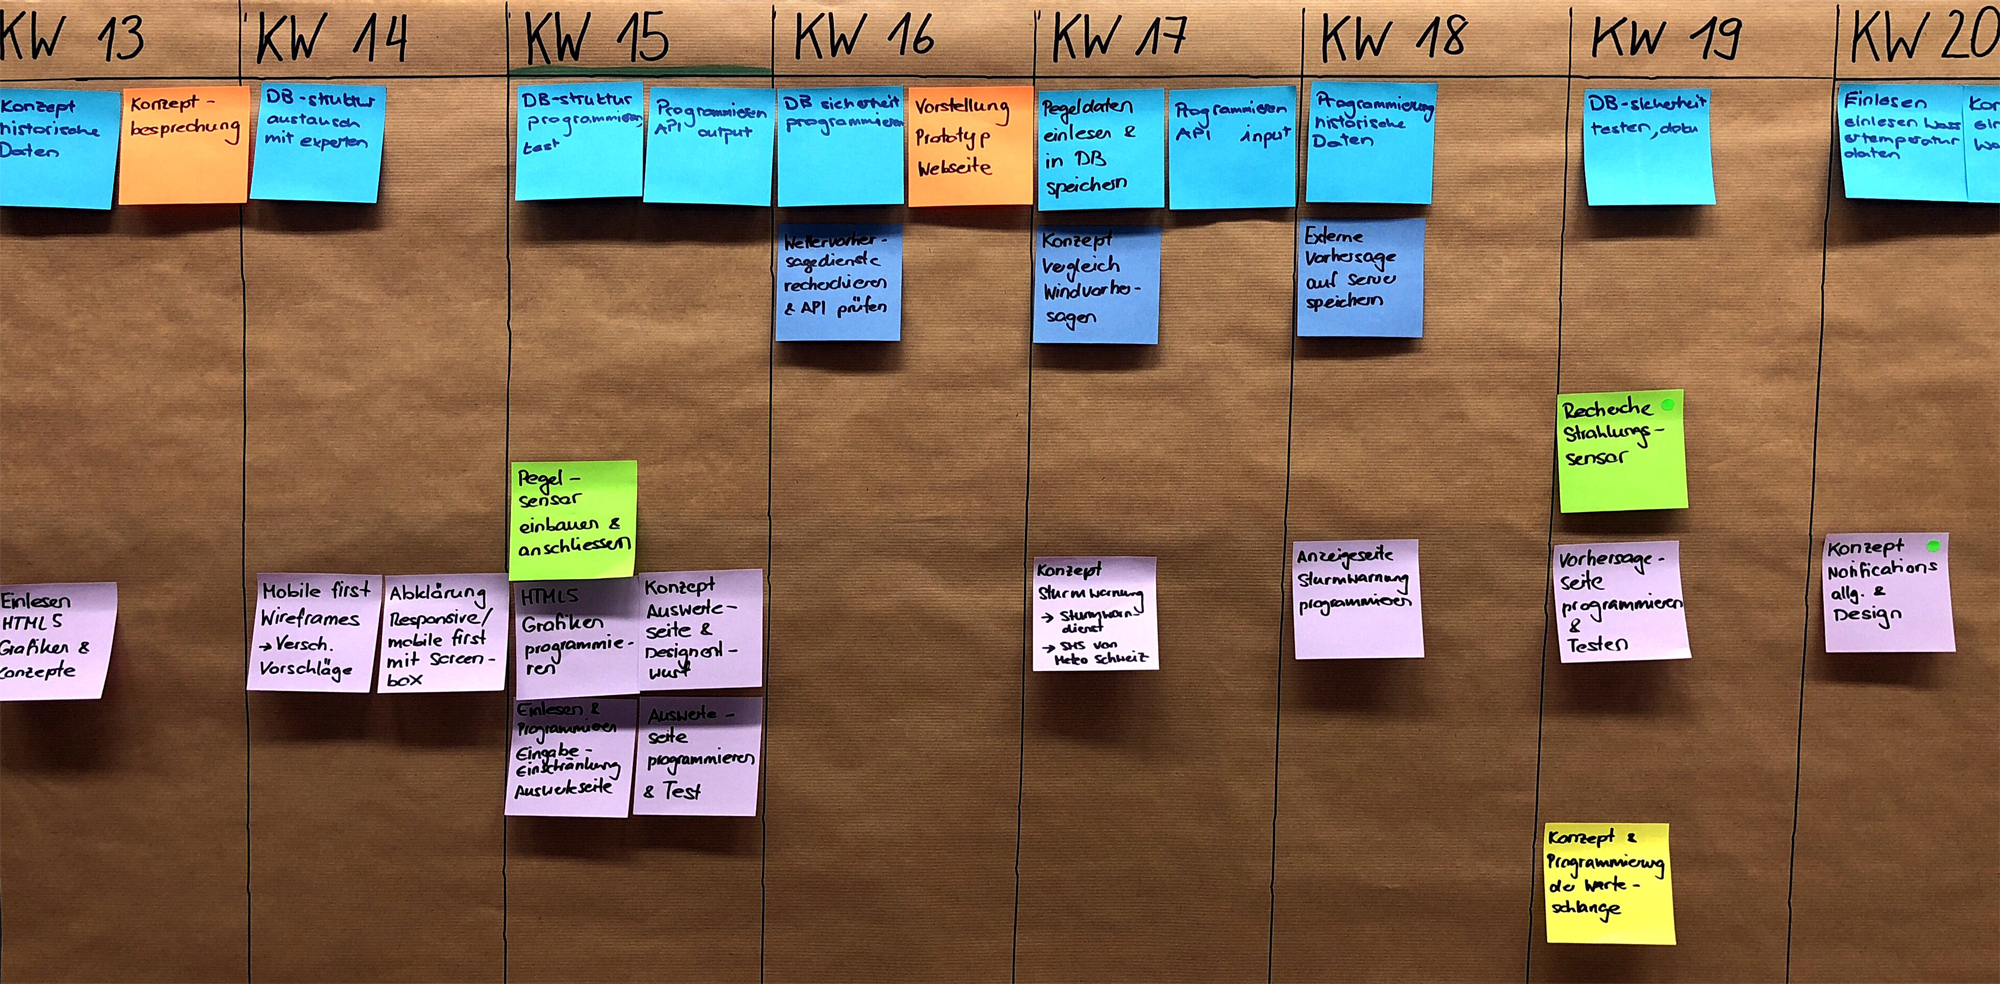
\includegraphics[angle=90,height=1\textheight,keepaspectratio]{img/terminplan.pdf}
\caption{Projektplan für die Bachelor-Arbeit}
\label{img:terminplan}
\end{figure}




\subsection{Dokumentation}

%Allgemein
Für die Bachelor-Arbeit verwenden wir unterschiedliche Dokumentationswerkzeuge. Bei der Auswahl haben wir darauf geachtet, das die Tools kostenlos nutzbar und für sämtliche Plattformen verfügbar sind (Windows, Mac, iPad, usw.). Weiter war uns wichtig, dass die Tools untereinander kommunizieren können. 

% github / Trello / Toggl
\subsubsection*{Versionierung und Zeiterfassung}
Sämtliche Artefakte speichern wir auf \textit{github}. Wir haben somit eine automatische Versionierung der Dokumente und können unabhängig voneinander an den Dokumenten arbeiten. Die Planung bzw. Darstellung des Entwicklungsprozesses erledigen wir mir \textit{Trello}. Es ist eine intuitive Webanwendung, welche diverse Integrationsmöglichkeiten mit den anderen Tools bietet. Für die Zeiterfassung verwenden wir \textit{Toggl}, welches mittels Plugin direkt in Trello integriert werden kann.

% Kommunikation nach aussen
\subsubsection*{Reporting; Kommunikation extern}
Damit wir keine Besprechungsprotokolle verschicken müssen und alle Informationen für alle immer zugänglich sind, haben wir entschieden, das Reporting in Form einer öffentlichen Webseite zu erstellen. github bietet mit \textit{GitPages} einen Hosting-Service an, der genau dies ermöglicht. Der Vorteil von \textit{GitPages} ist, dass wir sämtliche Daten in einem einzigen Ort bzw. Repository vereint haben. Damit wir uns nicht mit Formatierung herumschlagen müssen und uns auf den Inhalt konzentrieren können, verwenden wir \textit{mkdocs} als Template Engine. Die Webseiten-Einträge können wir dadurch auf simple Art in Form von Markdown-Files erstellen.

% Kommunikation nach innen
\subsubsection*{Kommunikation teamintern}
Innerhalb des Teams nutzen wir das Kommunikationstool \textit{Slack}. Dieses ermöglicht uns, Konversationen als Chat aufzuzeichnen und nach Themen zu gruppieren. Weiter lassen sich Dokumente austauschen. Sämtliche git-Posts werden von Slack automatisch geloggt und können, falls gewünscht, als push-Notification angezeigt werden.
Das wöchentliche Team-Meeting findet über \textit{Skype} statt, da wir den regelmässigen mündlichen Austausch als zentralen Punkt erachten.

% Bericht = LaTeX
\subsubsection*{Dokumentation}
Den Bericht werden wir in \LaTeX\ verfassen. Wir haben uns für \LaTeX\ entschieden, da wir uns auf den Inhalt konzentrieren können und das Layout automatisiert ist. Weiter ist \LaTeX\ in der Wissenschaft weit verbreitet. Die Bachelor-Arbeit ist deshalb eine gute Gelegenheit, uns in dieses Thema einzuarbeiten.




% braucht es das?
\FloatBarrier

\newpage
%%%%%%%%%%%%%%%%%%%%%%%%%%%%%%%%%%%
%%  Schluss
%%%%%%%%%%%%%%%%%%%%%%%%%%%%%%%%%%%
\section{Schluss}
% viele Konzepte
Während der Analyse der Wetterstation konnten wir diverse Schwachstellen ausfindig machen, die mehr oder weniger dringend beseitigt werden müssen.
Bei vielen Problemen muss zuerst ein Lösungskonzept erstellt werden, bevor mit der Behebung begonnen werden kann. Diese Arbeit bedarf einiges an Recherchearbeit und darf nicht unterschätzt werden.
\newline

\noindent
% unbekannte Thematik
Das gesamte Themengebiet von Barrierefreiheit und User Interface Design ist für uns neu und wir müssen das gesamt Know-how von Grund auf aufbauen. Ebenso ist die Arbeit mit Skripten und die Verdünnung der Daten auf einer Datenbank neu für uns. Auch hier ist ein grosser Teil für Einlesearbeiten zu erwarten.
\newline

\noindent
% schwierige Rahmenbedingungen
Als kritisch bezwiehungsweise schwer abschätzbar sehen wir die gegebenen Rahmenbedingung, die uns allenfalls in der Lösungsfindung stark einschränken.
Zum Beispiel ist dies das vorgegebene CMS oder die Schnittstelle zum Kombi-Wetter-Transmitter über \textit{WeatherDisplay}.
\newline

\noindent
% Rückblick auf Stundenschätzung
Anfangs Fachmodul schätzen wir die Stundenaufwände für die während dem Fachmodul anstehenden Arbeiten ab. Die effektiven Aufwände haben wir mittels Toggl dokumentier, sodass wir nun am Schluss des Fachmoduls die geleisteten Stunden den geplanten gegenüberstellen können. Die Auflistung befindet sich in Tabelle~\ref{plan-ist}. 
Sowohl die produktiven Arbeiten, d.h. die Arbeiten, die gemäss Fachmodul-Auftrag zu erledigen waren, als auch die Administrativen Aufwände für Meetings und Wochenreports stimmen recht gut. Der Aufwand für die Dokumentation hingegen haben wir unterschätzt. Wenn wir anfangs Bachelor-Arbeit den definitiven Terminplan erstellen müssen wir dies berücksichtigen.
\newline

\begin{table}[h]
\centering
\begin{tabular}{|l|l|l|l|}
\hline
 Tätigkeit			&  Plan	& Ist  	& Delta  		\\ \hline
 Produktive Arbeit	&  86		&  75		&  13~\%		\\ \hline
 Dokumentation		&  44		&  73		&  65~\%		\\ \hline
 Administration		&  30		&  27		&  10~\%		\\ \hline
\end{tabular}
\caption{Vergleich der Planstunden zu den Ist-Stunden}
\label{table:plan-ist}
\end{table}

\noindent
Zusammenfassend sehen wir Bachelor-Arbeit als machbar an. Zeitlich bleibt jedoch nicht viel Spielraum. Die grossen Unbekannten wie  einschränkende Rahmenbedingungen und schwer abzuschätzenden Aufwand für Einarbeitung und Konzepterstellung bedingen jedoch, dass der Fortschritt kontinuierlich und kritisch geprüft wird.
\section{Rechtliche Ansprüche}
siehe separates Dokument
\section{Verzichterklärung}
\newpage
\bibliography{literatur}{}	
\bibliographystyle{plain} 


\end{document}